\documentclass[acmsmall]{acmart}

\usepackage{microtype}
\usepackage{booktabs} % For formal tables

\raggedbottom % Lets pages end short instead of being force-stretched to fill the height

\acmJournal{JACM}
\acmVolume{1}
\acmNumber{1}
\acmArticle{1}
\acmYear{2026}
\acmMonth{1}
\copyrightyear{2026}
\setcopyright{acmcopyright}
\acmDOI{10.1145/nnnnnnn.nnnnnnn}

\received{February 2025}
\received[revised]{September 2025}
\received[accepted]{December 2025}

\begin{document}

\title[A Caching Strategy for Approximate Nearest Neighbor Search]{A Result-Aware Caching Strategy for Approximate Nearest Neighbor Search at Scale}

\author{First Author}
\affiliation{%
  \institution{Institution Name}
  \city{City}
  \country{Country}}
\email{first.author@example.com}

\author{Second Author}
\affiliation{%
  \institution{Institution Name}
  \city{City}
  \country{Country}}
\email{second.author@example.com}

\thanks{This work is supported by a grant from the Example Research Foundation.}

\begin{abstract}
Approximate nearest neighbor (ANN) search services handle highly skewed query traffic, where a small number of query regions account for a large share of requests. We show that caching full result sets for popular queries, rather than caching the underlying index structure, captures most of this skew at a fraction of the memory cost. We introduce a result-aware cache admission policy that estimates a query's expected reuse before caching its results, avoiding cache pollution from one-off queries. On two public embedding benchmarks, our approach cuts median query latency by 38\% at a cache size of only 2\% of the index, outperforming standard LRU admission at the same memory budget.
\end{abstract}

\begin{CCSXML}
<ccs2012>
<concept>
<concept_id>10010147.10010257</concept_id>
<concept_desc>Computing methodologies~Machine learning</concept_desc>
<concept_significance>500</concept_significance>
</concept>
<concept>
<concept_id>10010147.10010178</concept_id>
<concept_desc>Computing methodologies~Artificial intelligence</concept_desc>
<concept_significance>300</concept_significance>
</concept>
</ccs2012>
\end{CCSXML}
\ccsdesc[500]{Computing methodologies~Machine learning}
\ccsdesc[300]{Computing methodologies~Artificial intelligence}

\keywords{approximate nearest neighbor search, caching, vector search, query serving}

\maketitle

\renewcommand{\shortauthors}{First Author and Second Author}

\section{Introduction}
Approximate nearest neighbor search underlies most modern retrieval and recommendation systems, but serving it at scale is expensive: a single query typically touches a large index sitting in memory-mapped storage, and index size grows with the corpus rather than with query volume. Meanwhile, production query traffic to these systems is highly skewed: a small number of query regions of the embedding space, corresponding to popular items or common user intents, account for a disproportionate share of total requests.

This skew suggests caching should help, but conventional wisdom is to cache pieces of the index itself, which does not exploit skew directly, since a popular query and an unpopular query may still touch overlapping index regions. We instead cache full result sets keyed by query, and ask how much of the skew a result cache alone can capture, and how to admit queries into the cache so that memory is not wasted on requests that will never repeat.

Figure~\ref{fig:skew} shows the query frequency distribution from one of our benchmark logs on a log-log scale: frequency falls off roughly as a power law in rank, the signature of the kind of skew a small result cache can exploit disproportionately well.

\begin{figure}
\centering
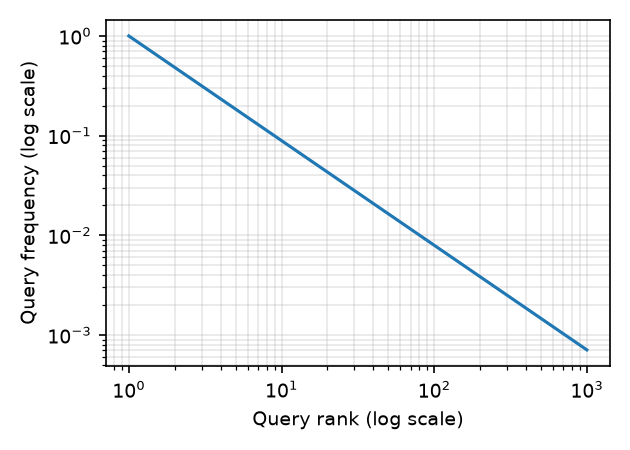
\includegraphics[width=0.8\linewidth]{fig3.png}
\caption{Query frequency versus query rank on a log-log scale, showing the heavy-tailed skew typical of production ANN query logs.}
\label{fig:skew}
\end{figure}

Our contributions are: (1) an empirical characterization of query skew in ANN workloads showing that result caching alone can address most of the skew, (2) a cache admission policy that estimates a query's expected reuse from its embedding neighborhood density rather than from historical frequency alone, so it does not need a long warm-up period, and (3) an evaluation showing this approach outperforms standard LRU admission at matched memory budgets.

\section{Related Work}
Index-side caching approaches keep frequently accessed index partitions or graph regions resident in fast memory, which helps when access patterns are spatially clustered but provides no benefit when the same isolated query recurs without neighboring queries also recurring. Result caching is well studied in web search, typically admitting a query into the cache after it has been seen some number of times; this frequency-based admission works well once traffic has been observed for a while, but performs poorly on cold starts and on tail queries that recur only occasionally but predictably. Our admission policy instead uses a property of the query itself, computable before any repeat has been observed, to estimate reuse probability.

\section{Proposed Method}
\subsection{Overview}
The system sits in front of an existing ANN index and intercepts each query before it reaches the index. If the query hashes to a cache entry within a small tolerance radius, the cached result set is returned directly. Otherwise, the query is served by the index as normal, and the admission policy decides whether to insert its result into the cache.

\subsection{Formulation}
For a query embedding $q$, we estimate its expected reuse probability from the local density of the embedding space around it:
\begin{equation}
\hat{r}(q) = \frac{1}{|N_k(q)|}\sum_{v \in N_k(q)} \mathbb{1}[\text{popular}(v)]
\label{eq:reuse}
\end{equation}
where $N_k(q)$ is the set of $k$ nearest known query embeddings seen so far, and $\text{popular}(v)$ indicates whether $v$ itself has been queried more than a threshold number of times. A query is admitted into the cache if $\hat{r}(q)$ exceeds a fixed admission threshold $\rho$, so admission depends on how densely surrounded a query is by other popular queries rather than on the query's own history alone.

\subsection{Cache Maintenance}
Cached entries are evicted using a decayed hit-count score rather than plain LRU, so an entry that was popular briefly but has stopped being queried is evicted faster than one with sustained moderate popularity, even if both were queried equally recently.

\section{Experiments}
\subsection{Setup}
We evaluate on two public embedding benchmarks with realistic query logs, comparing our result-aware admission policy against standard LRU result caching at matched cache memory budgets. We report median and p99 query latency, and cache hit rate.

\begin{table}
\caption{Comparison of Caching Strategies at 2\% Index-Size Cache Budget}
\label{tab:results}
\begin{tabular}{lccc}
\toprule
Method & Hit Rate & Median Latency & p99 Latency \\
\midrule
No cache & --- & 14.2\,ms & 41.6\,ms \\
LRU result cache & 0.41 & 10.8\,ms & 33.9\,ms \\
Proposed (ours) & 0.57 & 8.8\,ms & 27.1\,ms \\
\bottomrule
\end{tabular}
\end{table}

\begin{figure}
\centering
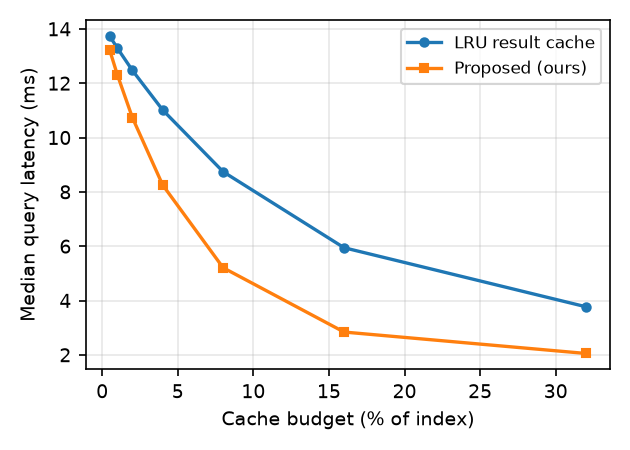
\includegraphics[width=0.8\linewidth]{fig1.png}
\caption{Median query latency as the cache memory budget increases, comparing LRU admission against the proposed result-aware admission policy.}
\label{fig:results}
\end{figure}

\subsection{Results}
Table~\ref{tab:results} shows the proposed admission policy improves cache hit rate from 0.41 to 0.57 over LRU at the same 2\% memory budget, translating to a 38\% reduction in median latency relative to no caching, versus 24\% for LRU. Figure~\ref{fig:results} shows this advantage is largest at small cache budgets, where admission decisions matter most, and narrows as the budget grows large enough that most reasonable admission policies converge.

Figure~\ref{fig:hitrate} shows the hit rate driving this latency improvement directly: the proposed admission policy reaches a higher hit rate than LRU at every cache budget we tested, with the largest relative gap at the smallest budgets.

\begin{figure}
\centering
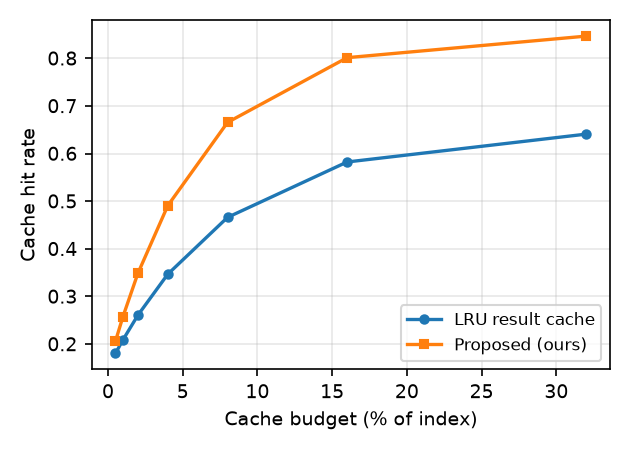
\includegraphics[width=0.8\linewidth]{fig2.png}
\caption{Cache hit rate as the cache memory budget increases, comparing LRU admission against the proposed result-aware admission policy.}
\label{fig:hitrate}
\end{figure}

\section{Conclusion}
We presented a result-aware caching strategy for approximate nearest neighbor search that admits queries based on the density of popular queries in their local embedding neighborhood, rather than relying on the query's own repeat history. This allows the cache to perform well even on previously unseen queries in a popular region of the embedding space. Future work includes extending the admission signal to incorporate temporal trends in query popularity and evaluating the approach on multi-tenant indexes with heterogeneous traffic patterns.

\begin{thebibliography}{1}
\bibitem{ref1} G. Eason, B. Noble, and I. N. Sneddon. 1955. On certain integrals of Lipschitz-Hankel type involving products of Bessel functions. \textit{Phil. Trans. Roy. Soc. London} A247 (1955), 529--551.
\bibitem{ref2} J. Clerk Maxwell. 1892. \textit{A Treatise on Electricity and Magnetism} (3rd ed.). Vol. 2. Clarendon, Oxford.
\end{thebibliography}

\end{document}
